%% ----------------------------------------------------------------
%% MAIN FILE (the one that you compile with LaTeX)
%% ---------------------------------------------------------------- 

% \documentclass[a4paper, 11pt, twoside, openright]{uis-thesis}
\documentclass[a4paper, 11pt]{uis-thesis}
\graphicspath{{figures/}}  % Location of the graphics files (set up for graphics to be in PDF format)

% Include any extra LaTeX packages required
\usepackage[square, numbers, comma, sort&compress]{natbib}  % Use the "Natbib" style for the references in the Bibliography
\usepackage{verbatim}  % Needed for the "comment" environment to make LaTeX comments
% \usepackage{vector}  % Allows "\bvec{}" and "\buvec{}" for "blackboard" style bold vectors in maths
\usepackage{algorithm}
\usepackage{algorithmic}
\usepackage[T1]{fontenc}
\usepackage{subfigure}
\usepackage{venturis2}
\usepackage{lmodern}
\usepackage{textcomp}    % solve issues with lmodern
\usepackage{amsfonts}
\usepackage{amsmath}
\usepackage{amsthm}
\usepackage{pdfpages}
\usepackage{microtype}   % better typesetting with pdfLaTeX
\usepackage[compact]{titlesec}
\usepackage{booktabs}
\usepackage{sectsty}     % section titles in specified font face

\allsectionsfont{\sffamily}
\numberwithin{algorithm}{chapter}
\setcounter{secnumdepth}{2}
\setcounter{tocdepth}{2}
\renewcommand{\captionlabelfont}{\sffamily\bfseries}
\newtheorem{thm}{Theorem}
\renewcommand{\algorithmicrequire}{\textbf{Input:}}
\renewcommand{\algorithmicensure}{\textbf{Output:}}
\hypersetup{urlcolor=blue, colorlinks=true}  % Colours hyperlinks in blue, but this can be distracting if there are many links.

\listfiles

%\usepackage[draft]{hyperref}
%\usepackage[hyperfootnotes=false,plainpages=false]{hyperref}
%% ----------------------------------------------------------------
\begin{document}
\frontmatter	  % Begin Roman style (i, ii, iii, iv...) page numbering
% Fill your name and supervisor name and sign it and replace the frontpage.
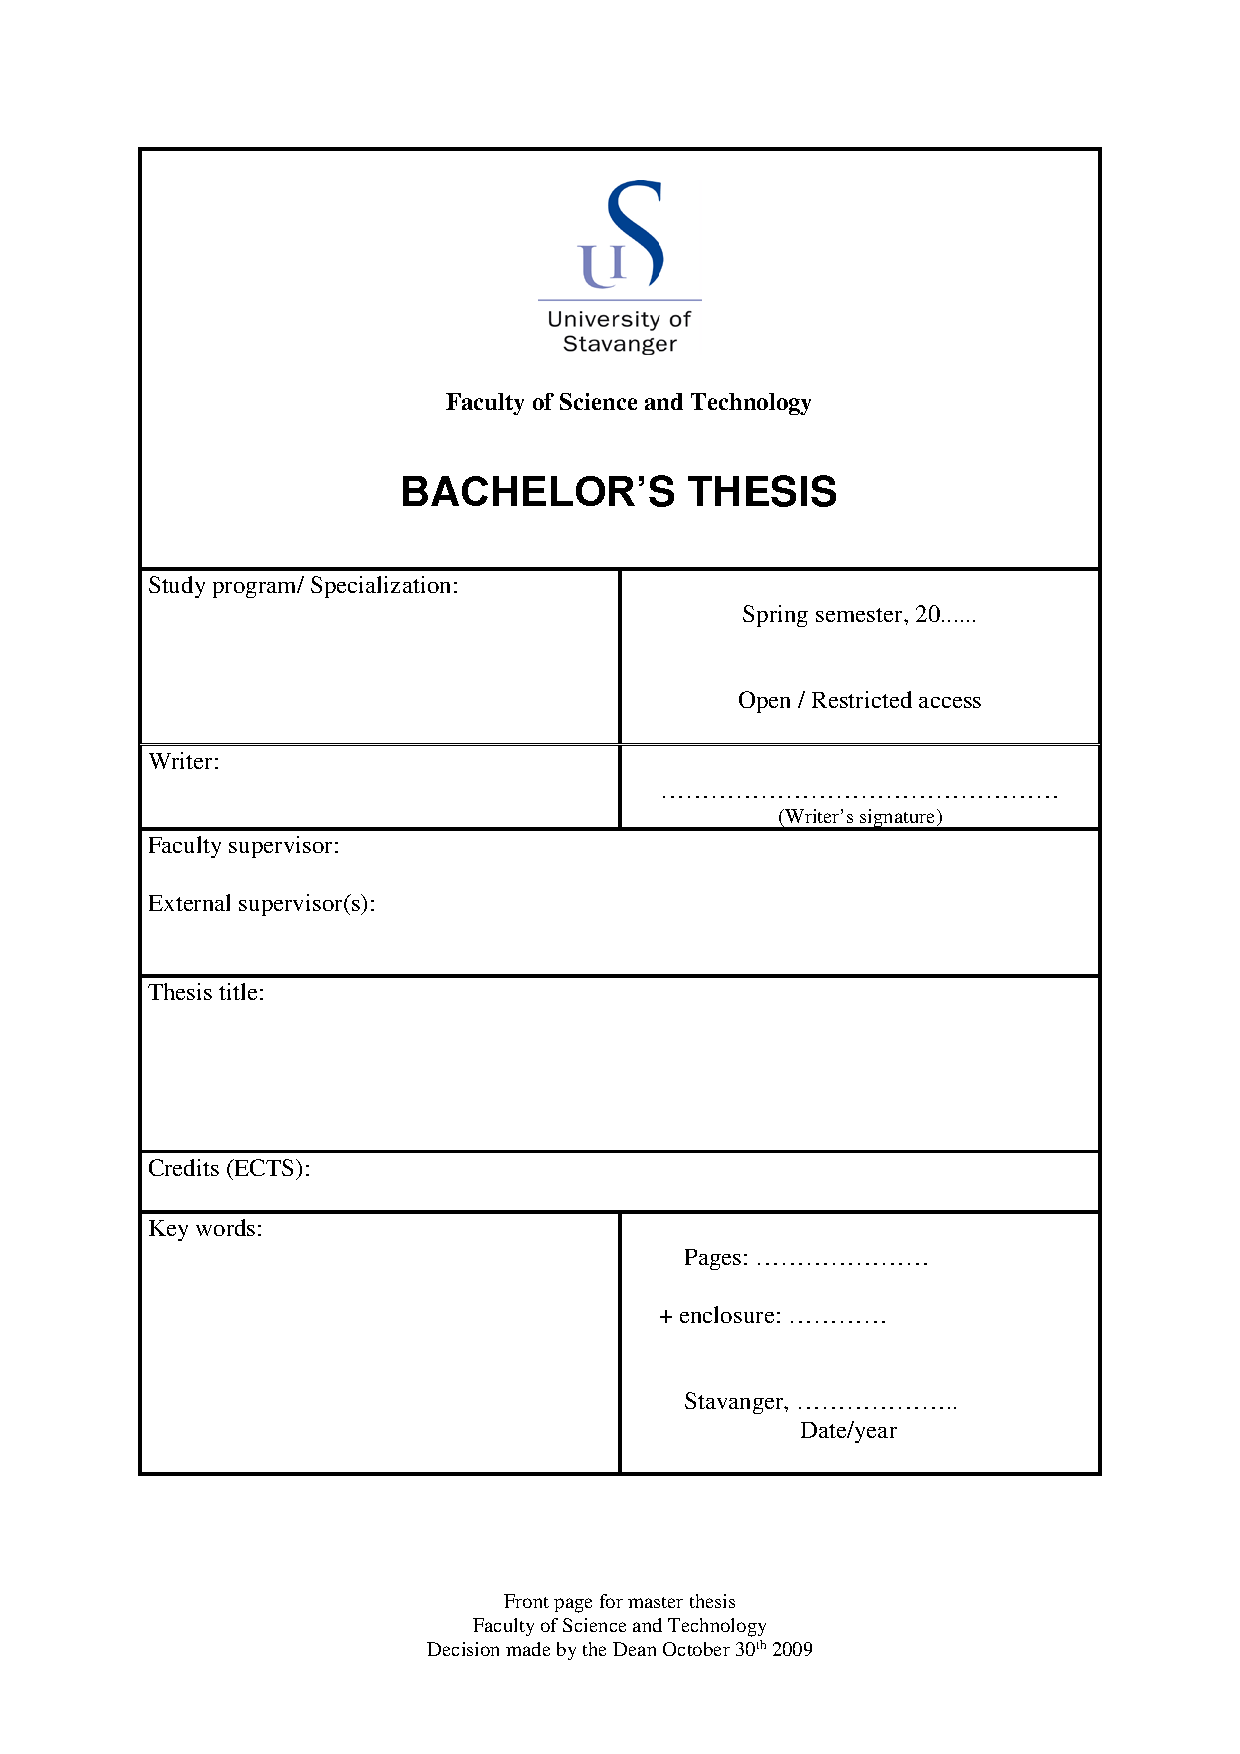
\includepdf[offset=25mm -25mm, scale=1]{./frontpage-bachelors.pdf}

% TODO(meling) Fix authors macro to allow multiple entries
% TODO(meling) Add supervisor macro and possibly other frontpage macros

\title{Thesis Title}
\authors{FirstName LastName and\\ AnotherName WithLastName}
\addresses{\groupname\\\deptname\\\univname}  % Do not change this here, instead these must be set in the "Thesis.cls" file, please look through it instead
\date       {\today}
\subject    {}
\keywords   {}

\maketitle
%% ----------------------------------------------------------------

\setstretch{1.3}  % It is better to have smaller font and larger line spacing than the other way round

% Define the page headers using the FancyHdr package and set up for one-sided printing
%\fancyhead{}  % Clears all page headers and footers
%\rhead{\thepage}  % Sets the right side header to show the page number
%\lhead{}  % Clears the left side page header

% \pagestyle{fancy}  % Finally, use the "fancy" page style to implement the FancyHdr headers
% \fancyhead[RE,LO]{\sffamily\bfseries\nouppercase{\rightmark}}
% \fancyhead[LE,RO]{\thepage}


%% ----------------------------------------------------------------
\pagestyle{empty}  % No headers or footers for the following pages
% % % Declaration Page required for the Thesis, your institution may give you a different text to place here
% \Declaration{

% \addtocontents{toc}{\vspace{1em}}  % Add a gap in the Contents, for aesthetics

%TODO: use macro for authors; if multiple, we should say "We" instead of "I"
% I, Vinay Setty, declare that this thesis titled, `Efficiently Identifying Interesting Time Points in Text Archives' and the work presented in it are my own. I confirm that:

% \begin{itemize} 
% \item[\tiny{$\blacksquare$}] This work was done wholly or mainly while in candidature for a master's degree at this University.
  
% \item[\tiny{$\blacksquare$}] Where I have consulted the published work of others, this is always clearly attributed.
 
% \item[\tiny{$\blacksquare$}] Where I have quoted from the work of others, the source is always given. With the exception of such quotations, this thesis is entirely my own work.
 
% \item[\tiny{$\blacksquare$}] I have acknowledged all main sources of help.

% \end{itemize}
%  \vspace{5pt}
% Signed:\\
% \rule[1em]{25em}{0.5pt}  % This prints a line for the signature
 
% Date:\\
% \rule[1em]{25em}{0.5pt}  % This prints a line to write the date
% }
% \clearpage  % Declaration ended, now start a new page

% \clearpage
\null\vfill
% Now comes the "Funny Quote", written in italics
\textit{``Programming is a nice break from thinking.''}

\begin{flushright}
Leslie Lamport
\end{flushright}

\vfill\vfill\vfill\vfill\vfill\vfill\null

\clearpage
\addtotoc{Abstract}  % Add the "Abstract" page entry to the Contents
\abstract{
\addtocontents{toc}{\vspace{1em}}  % Add a gap in the Contents, for aesthetics

}

\clearpage

\setstretch{1.3}  % Reset the line-spacing to 1.3 for body text (if it has changed)

% The Acknowledgements page, for thanking everyone
\acknowledgements{
\addtocontents{toc}{\vspace{1em}}  % Add a gap in the Contents, for aesthetics
I would like to thank my supervisors for their fantastic enthusiasm and help with writing this thesis. 

}

\clearpage

\tableofcontents

\setstretch{1.3}  % Return the line spacing back to 1.3

\addtocontents{toc}{\vspace{2em}}  % Add a gap in the Contents, for aesthetics

%% ----------------------------------------------------------------
\mainmatter	  % Begin normal, numeric (1,2,3...) page numbering
\pagestyle{fancy}  % Return the page headers back to the "fancy" style

% Include the chapters of the thesis, as separate files
% Just uncomment the lines as you write the chapters


\chapter{Introduction}
\label{ch:intro}

3-5 pages

\section{Background and Motivation}
\label{sec:background}
\begin{itemize}
    \item Awaken the reader's interest and convince her why the theme is important.
    \item Background information might be historical in nature, or it might refer to previous research or practical considerations.
    \item Provide an example or use case for the problem.
    \item It should be written on a level that it's understandable by anyone with a computer science bachelor's degree.
\end{itemize}

\section{Objectives}
\label{sec:objectives}
\begin{itemize}
   \item Define the goals of your study. It might be presented as a bullet list.
\end{itemize}


\section{Approach and Contributions}
\label{sec:approach}

\begin{itemize}
  \item Give a brief summary of your overall approach.
  \item Summarize the specific contributions that you made in this thesis (e.g., a task definition, a method or model, a test collection, empirical results, analysis, etc.). It might be presented as a bullet list.
\end{itemize}

\section{Outline}
\begin{itemize}
    \item Give an overview of the main points and the structure of your thesis. ``Chapter 2 covers ... Chapter 3 describes ... ''
    \item Show in a natural way how the different parts (chapters) relate to each other.
\end{itemize}

\chapter{Background}
\label{ch:background}
10 - 15 pages

\begin{itemize}
   \item An alternative heading is "Technology and tools".
Detail your choice of technology and development tools (typically, each in a separate section).
   \item Show how the particular choice of technology and tools is suited to reach your objectives, and demonstrate that you have given due consideration to the suitability of them (e.g., by discussing alternatives and presenting a feature comparison table).
   \item If there is related work done by others (e.g., similar tools or systems), discuss it and explain how yours relates to it.
   \item Mind that the reader may have never heard about these things. You need to discuss them in such detail that it is possible to follow later parts of the thesis without having to consult external resources.
    \item Key concept / tool / technology 1
    \item Key concept / tool / technology 2
    \item ...
    \item To include reference use Bibtex as below:
    \begin{itemize}
    \item Use \verb|\citet{}| for textual citation. For example, \citet{Balog:2018:Book} proposed...
    \item Use \verb|\citep{}| for parenthetical citation. For example, In \citep{Zhang:2020:KDD} the idea of ..
    \item Here is an example of a PhD thesis:  \citet{Maxwell:2019:PhDThesis} 
    \item Here is how a Journal article would look in the Bibliography: \citet{Sanderson:2010:FnTIR}
    \item Never write out Smith et al., there is a \verb|\citeauthor{}| command for that (but most likely what you're looking for is actually \verb|\citet{}|).
    \end{itemize}
\end{itemize}


\chapter{Approach}
\label{ch:approach}
20 - 30 pages
\begin{itemize}
    \item This chapter describes your main contributions (i.e., what you did) and the decisions that went into them (i.e., why did you did it the way you did it).
    
\end{itemize}
\section{Analysis and Requirements}
Describe the analysis of the problem and the specific requirements.

\section{Overview}
\begin{itemize}
    \item This section should explain the high-level design
    \item Include possibly an architecture figure that shows how the different parts fit together and what processing/technology/tools/datasets have been used for the different components.
\end{itemize}
    
    Name these themes based on the different components or sub-problems you are solving in your thesis.
    
    \section{Component 1}
    \section{Component 2}
    
    \begin{itemize}
    \item For larger/more complex projects, the separate components may be chapters on their own chapters on their own (e.g., back-end vs. front-end).
    \item Include screenshots, examples, tables, algorithms (with pseudo code), plots for some preliminary observations leading to some aspect of your approach decisions, etc. so that it's not just text.
    \item Always discuss the alternatives considered and the rationale for the choosing the solutions you adopted.
    \item You may include code snippets for interesting/challenging (sub)problems, but it is not the idea to walk through the source code line-by-line.
\end{itemize}
    

\chapter{Results}
\label{ch:eval}
5 - 15 pages
\begin{itemize}
\item Alternative heading: ``Testing and Validation''.
\item Present your results, and provide an analysis of them. Results can be quantitative and/or qualitative (from benchmark, user study, user satisfaction survey, etc.).
\item It is desired that you have some results, nevertheless, this may not be applicable to all types of theses.
\end{itemize}

\section{Methodology}
Explain the methodology used for collecting results and the metrics used for evaluation.

\section{Experimental Results}
\begin{itemize}
    \item Present the results, using tables and (pretty) plots.
\end{itemize}

\section{Analysis}
Now that you presented the results, what do these results actually mean (esp. regarding the objectives you set out in the introduction)? Can you identify success and failure cases? What do the results say for individual parts you evaluate and overall in combination? Make sure you formulate clear take-home messages.


\chapter{Conclusions}
\label{ch:conclusion}
3-5 pages
\begin{itemize}
    \item Summary of the work you have done, what worked and what didn't
    \item Make sure it connects well with the Introduction.
\end{itemize}

\section{Future Directions}
Discuss potential future work that may fill gaps in your work, or approaches that seem promising to overcome problems you encountered but that you weren't able to tackle.

%% ----------------------------------------------------------------
% Now begin the Appendices, including them as separate files

\addtocontents{toc}{\vspace{2em}} % Add a gap in the Contents, for aesthetics

\appendix % Cue to tell LaTeX that the following 'chapters' are Appendices

\chapter{Instructions to Compile and Run System}
\label{apx:instructions}

\instructions{
This appendix may contain following:
%
\begin{itemize}
    \item Installation instructions
    \item Source code / class structure
    \item More detailed evaluation results
\end{itemize}
}


\addtocontents{toc}{\vspace{2em}}  % Add a gap in the Contents, for aesthetics
\backmatter

%% ----------------------------------------------------------------
\label{Bibliography}
\lhead{\emph{Bibliography}}  % Change the left side page header to "Bibliography"
\bibliographystyle{unsrtnat}  % Use the "unsrtnat" BibTeX style for formatting the Bibliography
\bibliography{Bibliography}  % The references (bibliography) information are stored in the file named "Bibliography.bib"

\end{document}
